
\documentclass[12pt, a4paper]{report}
\usepackage{epsfig}
\usepackage{subfigure}
%\usepackage{amscd}
\usepackage{amssymb}
\usepackage{graphicx}
%\usepackage{amscd}
\usepackage{amssymb}
\usepackage{subfiles}
\usepackage{framed}
\usepackage{subfiles}
\usepackage{amsthm, amsmath}
\usepackage{amsbsy}
\usepackage{framed}
\usepackage[usenames]{color}
\usepackage{listings}
\lstset{% general command to set parameter(s)
	basicstyle=\small, % print whole listing small
	keywordstyle=\color{red}\itshape,
	% underlined bold black keywords
	commentstyle=\color{blue}, % white comments
	stringstyle=\ttfamily, % typewriter type for strings
	showstringspaces=false,
	numbers=left, numberstyle=\tiny, stepnumber=1, numbersep=5pt, %
	frame=shadowbox,
	rulesepcolor=\color{black},
	,columns=fullflexible
} %
%\usepackage[dvips]{graphicx}
\usepackage{natbib}
\bibliographystyle{chicago}
\usepackage{vmargin}
% left top textwidth textheight headheight
% headsep footheight footskip
\setmargins{3.0cm}{2.5cm}{15.5 cm}{22cm}{0.5cm}{0cm}{1cm}{1cm}
\renewcommand{\baselinestretch}{1.5}
\pagenumbering{arabic}
\theoremstyle{plain}
\newtheorem{theorem}{Theorem}[section]
\newtheorem{corollary}[theorem]{Corollary}
\newtheorem{ill}[theorem]{Example}
\newtheorem{lemma}[theorem]{Lemma}
\newtheorem{proposition}[theorem]{Proposition}
\newtheorem{conjecture}[theorem]{Conjecture}
\newtheorem{axiom}{Axiom}
\theoremstyle{definition}
\newtheorem{definition}{Definition}[section]
\newtheorem{notation}{Notation}
\theoremstyle{remark}
\newtheorem{remark}{Remark}[section]
\newtheorem{example}{Example}[section]
\renewcommand{\thenotation}{}
\renewcommand{\thetable}{\thesection.\arabic{table}}
\renewcommand{\thefigure}{\thesection.\arabic{figure}}
\title{Research notes: linear mixed effects models}
\author{ } \date{ }


\begin{document}
	\author{Kevin O'Brien}
	\title{Mixed Models for Method Comparison Studies}
	\tableofcontents
	
	%----------------------------------------------------------------------------------------%
	\newpage
	\chapter{Current Methodologies: Bland-Altman Analysis}
	\section{Bland-Altman Methodology}
	
	%		\citet{BA83} highlighted the inadequacies of these approaches for comparing two methods of measurement, and proposed methodologies with this specific application in mind. Although the authors also acknowledge the opportunity to apply other, more complex, approaches, but argue that simpler approaches is preferable, especially when the
	%		results must be `explained to non-statisticians'.
In light of shortcomings associated with scatterplots, \citet*{BA83} recommend a further analysis of the data. Firstly
differences of measurements of two methods on the same subject should  be calculated, and then the average of those measurements
(Table 2.1). These differences and averages are then plotted (Figure ~\ref{GrubbsBA-noLOA}).

		
	The issue of whether two measurement methods comparable to the 	extent that they can be used interchangeably with sufficient accuracy is encountered frequently in scientific research. Statisticians Martin Bland and Douglas Altman recognized the inadequacies of several analyzes and articulated quite thoroughly the basis on which of which they are unsuitable for comparing two methods of measurement \citep*{BA83}, while instead recommended the use of graphical techniques to assess agreement.
	
In 1986 Bland and Altman published a paper in the Lancet proposing the difference plot for use for method comparison purposes. Bland Altman have recommended the use of graphical techniques to assess agreement. Principally their method is calculating, for each pair of corresponding two methods of measurement of some underlying quantity, with no replicate measurements, the difference $d_i$ and mean $a_i$. 	case-wise differences of measurements of two methods $d_{i} =
y_{1i}-y_{2i}, \mbox{ for }i=1,2,\dots,n$, on the same subject
should be calculated, and then the average of those measurements, 
($a_{i} = (y_{1i} + y_{2i})/2 \mbox{ for }i=1,2,\dots, n$. An important requirement is that the	two measurement methods use the same scale of measurement. Following a technique known as the Tukey mean-difference plot, as noted by \citet{kozak2014including}
	\citet{BA83} proposed that $a_i$ should be plotted against $d_i$, a plot now widely known as the Bland-Altman plot, and motivated this plot as follows:
	\begin{quote}
		``From this type of plot it is much easier to assess the magnitude
		of disagreement (both error and bias), spot outliers, and see
		whether there is any trend, for example an increase in (difference) for high values. This way of plotting the data is a very powerful way of displaying the results of a method comparison study."
	\end{quote}
	
	The case wise-averages capture several aspects of the data, such as expressing the range over which the values were taken, and assessing whether the assumptions of constant variance holds. Case-wise averages also allow the case-wise differences to be presented on a two-dimensional plot, with better data visualization qualities than a one dimensional plot. \citet{BA86}
	cautions that it would be the difference against either measurement value instead of their average, as the difference relates to both value. This approach has proved very popular, and the Bland-Altman plots is widely regarded as powerful graphical tool for making a visual assessment of the data.
	
	The magnitude of the inter-method bias between the two methods is simply the average of the differences $\bar{d}$. This inter-method bias is represented with a line on the Bland-Altman plot. As the objective of the Bland-Altman plot is to advise on the agreement of two methods, the individual case-wise differences are also particularly relevant. The variances around this bias is estimated by the standard deviation of these differences $S_{d}$. Further to this method, the presence of constant bias may be
	indicated if the average value differences is not equal to zero. \citet{BA86} does, however, indicate the indication of absence of bias does not provide sufficient information to allow a	judgement as to whether or not one method can be substituted for
	another.
	
	
		Furthermore they proposed their simple methodology specifically constructed for method comparison studies. They acknowledge that there are other valid, but complex, methodologies, and argue that
		a simple approach is preferable to this complex approaches,
		\emph{especially when the results must be explained to
			non-statisticians} \citep*{BA83}.
		
		

	
	
	Notwithstanding previous remarks about linear regression, the first step recommended, which the authors argue should be mandatory, is construction of a simple scatter plot of the data. The line of equality should also be shown, as it is necessary to give the correct interpretation of how both methods compare. In the case of good agreement, the observations would be distributed closely along the line of equality. In the case of good agreement, the observations would be distributed closely along this line. However, they are not useful for a thorough examination of the data. \citet{BritHypSoc} notes that data points will tend to cluster around the line of equality, obscuring interpretation. A scatter plot of the Grubbs data is shown in Figure ~\ref{GrubbsScatter}. Visual inspection confirms the previous conclusion that inter-method bias is present, i.e. the Fotobalk device has a tendency to record a lower velocity.
	
	\begin{figure}[h!]
		\begin{center}
			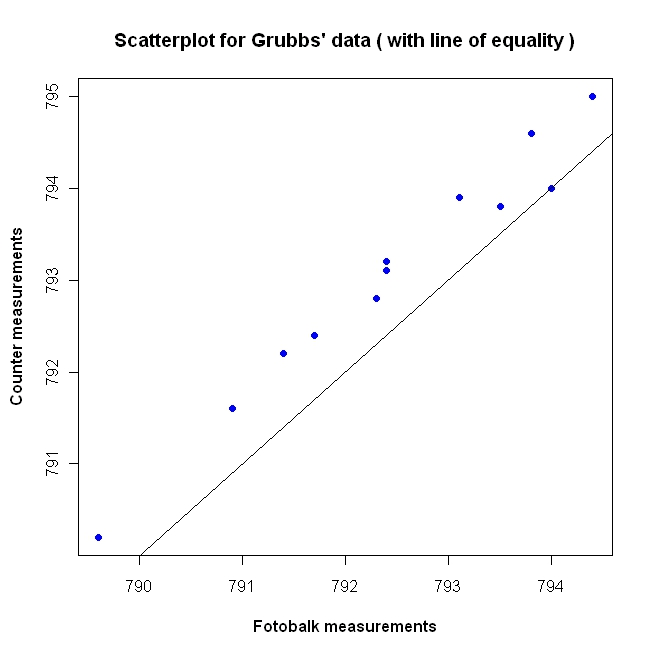
\includegraphics[width=125mm]{images/GrubbsScatter.jpeg}
			\caption{Scatter plot for Fotobalk and Counter methods.}\label{GrubbsScatter}
		\end{center}
	\end{figure}
	% %	\section{Variations and Alternative Graphical Methods}
	%In this section, we will look at some variations and enhancements of the Bland-Altman plot, as well as some alternative graphcial techniques. 
	% %	Strictly speaking, 
	The Identity Plot is advised by Bland and Altman as a prior analysis to the Bland-Alman plot, and therefore is neither a variant nor an alternative approach. However it is worth mentioning, as it is a simple, powerful and elegant technique that is often overlooked in method comparison studies. The identity plot is a simple scatter-plot approach of measurements for both methods on either axis, with the line of equality (the $X=Y$ line, i.e. the 45 degree line through the origin). This plot can gives the analyst a cursory examination of how well the measurement methods agree. In the case of good agreement, the covariates of the plot accord closely with the line of equality.

	%=============================================================================================== %
	%
	%	\section*{Rendering a Bland-Altma plot}
	%	Construction of a Bland-Altman plot can be implemented easily with \texttt{R} packages such as Bendix Carstensen's \texttt{MethComp} package, which is designed to \textit{provide computational tools to manipulate, display and analyze data from method comparison studies} \citep{BXC2010}.
	%	
	\section{Bland Altman Plots}



	
	
The Bland-Altman plot for comparing the `Fotobalk' and `Counter' methods, which shall henceforth be referred to as the `F vs C' comparison, is depicted in Figure ~\ref{GrubbsBA-noLOA}, using data from Table 1.3. The dashed line in . alludes to the inter method bias between the two methods, as mentioned previously. Bland and Altman
	recommend the estimation of inter method bias by calculating the
	average of the differences. In the case of Grubbs data the inter
	method bias is $-0.6083$ metres per second.

	

By inspection of the plot, it is also possible to compare the precision of each method. Noticeably the differences tend to increase as the averages increase.
		

	
\subsection{Bland-Altman plots for the Grubbs data}

	


	%================================================================================================= %		
	%Later it will be shown that case-wise differences are the sole
	%component of the next part of the methodology, the limits of
	%agreement.
	
	
	\begin{table}[h!]
		\renewcommand\arraystretch{0.7}%
		\begin{center}
			\begin{tabular}{|c||c|c||c|c|}
				\hline
				Round & Fotobalk  & Counter  & Differences  & Averages  \\
				&  [F] & [C] & [F-C] &  [(F+C)/2] \\
				\hline
				1 & 793.8 & 794.6 & -0.8 & 794.2 \\
				2 & 793.1 & 793.9 & -0.8 & 793.5 \\
				3 & 792.4 & 793.2 & -0.8 & 792.8 \\
				4 & 794.0 & 794.0 & 0.0 & 794.0 \\
				5 & 791.4 & 792.2 & -0.8 & 791.8 \\
				6 & 792.4 & 793.1 & -0.7 & 792.8 \\
				7 & 791.7 & 792.4 & -0.7 & 792.0 \\
				8 & 792.3 & 792.8 & -0.5 & 792.5 \\
				9 & 789.6 & 790.2 & -0.6 & 789.9 \\
				10 & 794.4 & 795.0 & -0.6 & 794.7 \\
				11 & 790.9 & 791.6 & -0.7 & 791.2 \\
				12 & 793.5 & 793.8 & -0.3 & 793.6 \\
				\hline
			\end{tabular}
			\caption{Fotobalk and Counter methods: Differences and Averages.}
		\end{center}
	\end{table}
	
	\begin{table}[h!]
		\renewcommand\arraystretch{0.7}%
		\begin{center}
			\begin{tabular}{|c||c|c||c|c|}
				\hline
				Round & Fotobalk  & Terma  & Differences  & Averages  \\
				&  [F] & [T] & [F-T] &  [(F+T)/2] \\
				\hline
				1 & 793.8 & 793.2 & 0.6 & 793.5 \\
				2 & 793.1 & 793.3 & -0.2 & 793.2 \\
				3 & 792.4 & 792.6 & -0.2 & 792.5 \\
				4 & 794.0 & 793.8 & 0.2 & 793.9 \\
				5 & 791.4 & 791.6 & -0.2 & 791.5 \\
				6 & 792.4& 791.6 & 0.8 & 792.0 \\
				7 & 791.7 & 791.6 & 0.1 & 791.6 \\
				8 & 792.3 & 792.4 & -0.1 & 792.3 \\
				9 & 789.6 & 788.5 & 1.1 & 789.0 \\
				10 & 794.4 & 794.7 & -0.3 & 794.5 \\
				11 & 790.9 & 791.3 & -0.4 & 791.1 \\
				12 & 793.5 & 793.5 & 0.0 & 793.5 \\
				
				\hline
			\end{tabular}
			\caption{Fotobalk and Terma methods: Differences and Averages.}
		\end{center}
	\end{table}
	
	\newpage
	
	\begin{figure}[h!]
		\begin{center}
			\includegraphics[width=120mm]{images/GrubbsBAplot-noLOA.jpeg}
			\caption{Bland-Altman plot For Fotobalk and Counter methods.}\label{GrubbsBA-noLOA}
		\end{center}
	\end{figure}
	
	
	
	In Figure 1.3 Bland-Altman plots for the `F vs C' and `F vs T'
	comparisons are shown, where `F vs T' refers to the comparison of
	the `Fotobalk' and `Terma' methods. Usage of the Bland-Altman plot
	can be demonstrate in the contrast between these comparisons. By inspection, there exists a larger inter-method bias in the `F vs C' comparison than in the `F vs T' comparison. Conversely there
	appears to be less precision in `F vs T' comparison, as indicated
	by the greater dispersion of covariates.
	
	\begin{figure}[h!]
		\begin{center}
			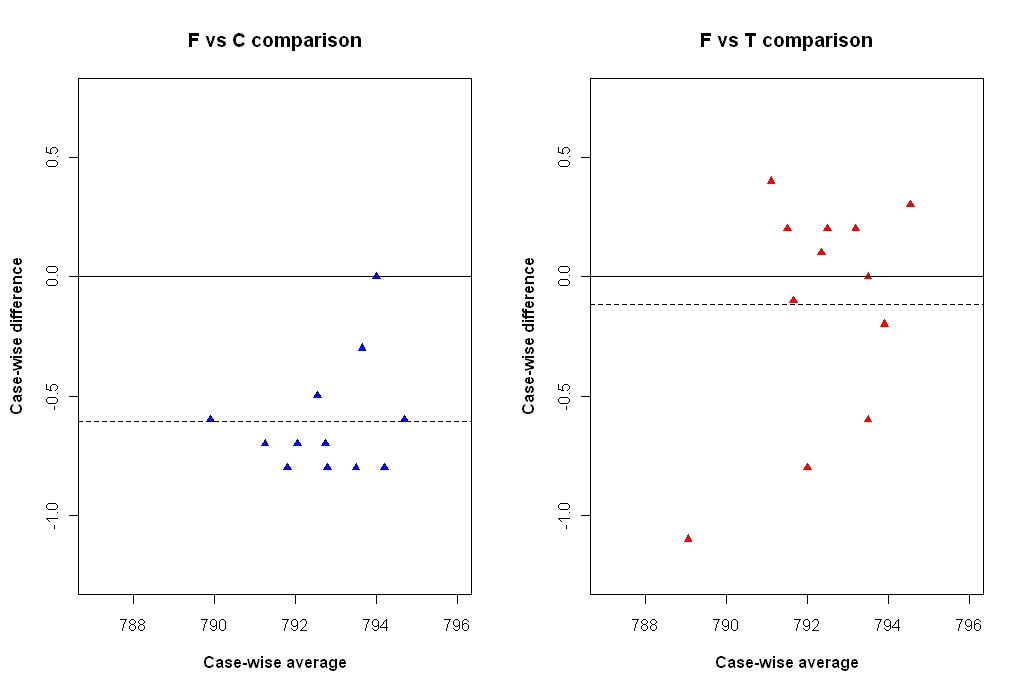
\includegraphics[height=60mm]{images/GrubbsDataTwoBAplots.jpeg}
			\caption{Bland-Altman plots for Grubbs' F vs C and F vs T comparisons.}\label{GrubbsDataTwoBAplots}
		\end{center}
	\end{figure}
	
	\newpage
	
	
	%\subfile{TechAcceptModel.tex}
	
	
	%\begin{figure}[h!]
	%	\begin{center}
	%		\includegraphics[width=120mm]{GrubbsBAplot-noLOA.jpeg}
	%		\caption{Bland-Altman plot For Fotobalk and Counter methods.}\label{GrubbsBA-noLOA}
	%	\end{center}
	%\end{figure}
	
	
	
	%	\section{scatter plots} The authors advise the
	%	use of scatter plots to identify outliers, and to determine if
	%	there is curvilinearity present. In the region of linearity
	%	,simple linear regression may yield results of interest.
	


	\subsection{Inspecting the Data}
	Bland-Altman plots are a powerful graphical methodology for making
	a visual assessment of the data. \citet*{BA83} express the
	motivation for this plot thusly:
	\begin{quote}
		"From this type of plot it is much easier to assess the magnitude
		of disagreement (both error and bias), spot outliers, and see
		whether there is any trend, for example an increase in
		(difference) for high values. This way of plotting the data is a
		very powerful way of displaying the results of a method comparison
		study."
	\end{quote}
Estimates for inter-method bias and variance of differences are only meaningful if there is uniform inter-bias and variability throughout the range of measurements. Fulfilment of these assumptions can be checked by visual inspection of the plot.The prototype Bland-Altman plots depicted in Figures 1.4, 1.5 and 1.6 are derived from simulated data, for the purpose of demonstrating how the plot would inform an analyst of features that would adversely affect use of the recommended approach.
	
	Figures ~\ref{BAFanEffect}, ~\ref{PropBias} and ~\ref{BAOutliers} are three Bland-Altman plots derived from
	simulated data, each for the purpose of demonstrating how the plot would inform an analyst of trends that would adversely affect use of the recommended methodology. Figure ~\ref{BAFanEffect} demonstrates how the Bland-Altman plot would indicate
	increasing variance of differences over the measurement range.
	Fitted regression lines, for both the upper and lower half of the
	plot, has been added to indicate the trend. Application of regression techniques to the Bland-Altman plot, and subsequent formal testing for the constant variability of differences is informative. The data set may be divided into two subsets, containing the observations wherein the difference values are less than and greater than the inter-method bias respectively. For both of these fits, hypothesis tests for the respective slopes can be performed. While both tests could be considered separately, multiple comparison procedures, such as the Benjamini-Hochberg \citep{BH} test, are advisable.
	
	Figure ~\ref{PropBias} is an example
	of cases where the inter-method bias changes over the measurement range. This is known as proportional bias, and is defined by \citet{ludbrook97} as meaning that `one method gives
	values that are higher (or lower) than those from the other by an
	amount that is proportional to the level of the measured variable'.
	
	\begin{figure}[h!]
		\begin{center}
			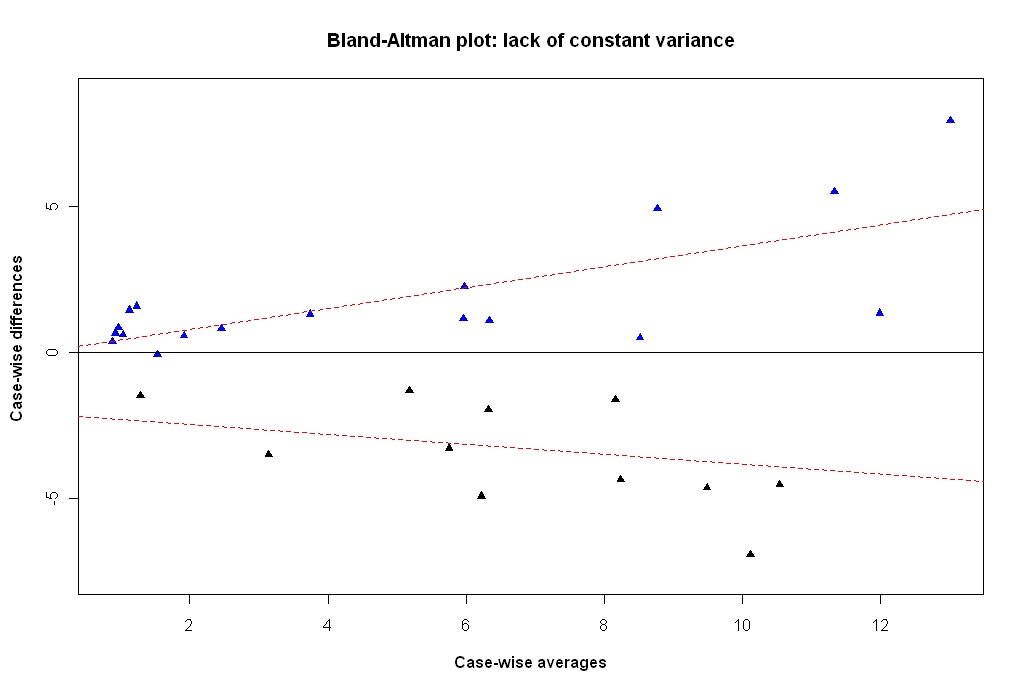
\includegraphics[width=110mm]{images/BAFanEffect.jpeg}
			\caption{Bland-Altman Plot demonstrating the increase of variance over the range}\label{BAFanEffect}
		\end{center}
	\end{figure}
	
	\begin{figure}[h!]
		\begin{center}
			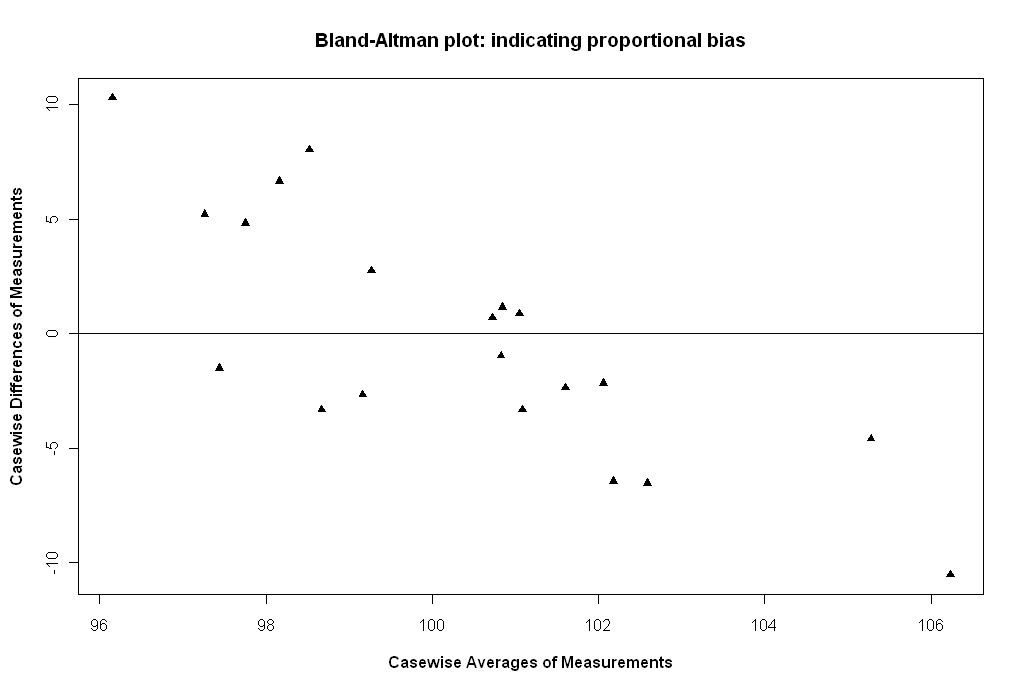
\includegraphics[width=110mm]{images/PropBias.jpeg}
			\caption{Bland-Altman Plot indicating the presence of proportional bias}\label{PropBias}
		\end{center}
	\end{figure}
Both of these cases violate the assumptions necessary for further analysis using limits of agreement, which shall be discussed later. The plot also can be used to identify	outliers. An outlier is an observation that is numerically distant from the rest of the data. Classification thereof is a subjective decision in any analysis, but must be informed by the logic of the formulation. Figure ~\ref{BAOutliers} is a Bland Altman plot with two
	conspicuous observations, at the extreme left and right of the
	plot respectively.
	
	
	\begin{figure}[h!]
		\begin{center}
			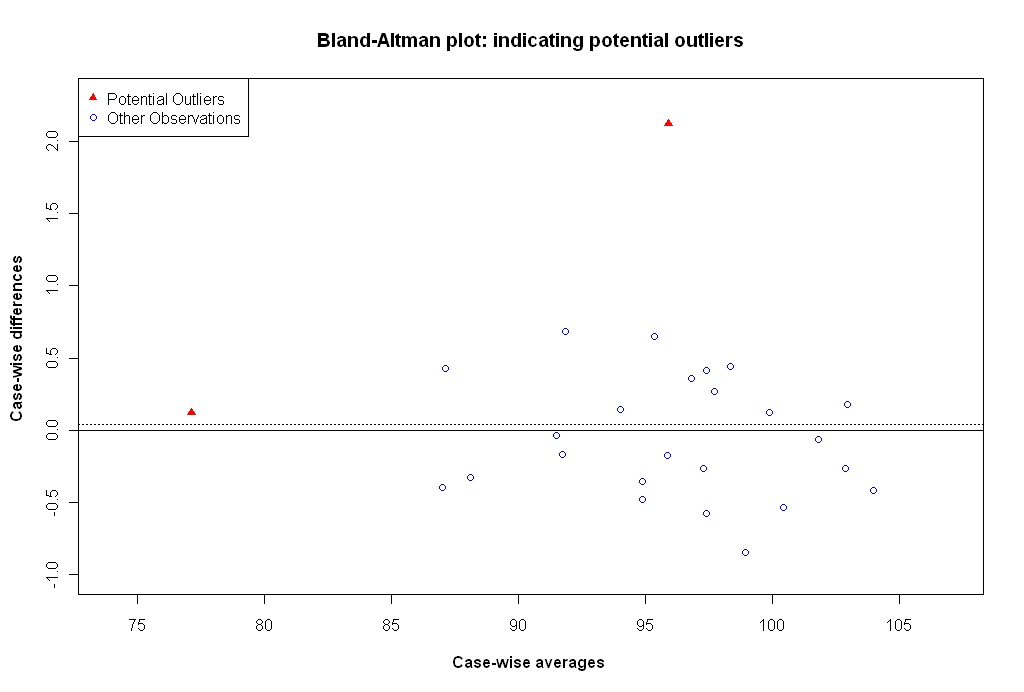
\includegraphics[width=125mm]{images/BAOutliers.jpeg}
			\caption{Bland-Altman Plot indicating the presence of Outliers}\label{BAOutliers}
		\end{center}
	\end{figure}
	
In the Bland-Altman plot, the horizontal displacement of any observation is supported by two independent measurements. Hence any observation , such as the one on the extreme right of figure ~\ref{BAOutliers}, should not be considered an outlier on the basis of a noticeable horizontal displacement from the main cluster. The one	on the extreme left should be considered an outlier, as it has a
noticeable vertical displacement from the rest of the observations.
	
\citet*{BA99} do not recommend excluding outliers from analyses. However recalculation of the inter-method bias estimate , and further calculations based upon that estimate, are useful for assessing the influence of outliers.\citep{BA99} states that \emph{"We usually find that this method of analysis is not too sensitive to one or two large outlying differences."}


\subsection{Detection of Outliers}
In their 1983 paper they merely state that the plot can be used to
'spot outliers'.In  their 1986 paper, Bland and Altman give an example of an
outlier. They state that it could be omitted in practice, but make
no further comments on the matter. In Bland and Altmans 1999 paper, we get the clearest indication of
what Bland and Altman suggest on how to react to the presence of
outliers. Their recommendation is to recalculate the limits
without them, in order to test the difference with the calculation
where outliers are retained.

BAExample -	The span has reduced from 77 to 59 mmHg, a noticeable but not
particularly large reduction.However, they do not recommend removing outliers. Furthermore, they say:

\textit{We usually find that this method of analysis is not too sensitive
	to one or two large outlying differences.}

We ask if this would be so in all cases. Given that the limits of
agreement may or may not be disregarded, depending on their
perceived suitability, we examine whether it would possible that
the deletion of an outlier may lead to a calculation of limits of
agreement that are usable in all cases?

Should an Outlying Observation be omitted from a data set? In
general, this is not considered prudent. Also, it may be required that the outliers are worthy of particular attention themselves.

Classifying outliers and recalculating We opted to examine this
matter in more detail. The following points have to be considered how to suitably identify an outlier (in a generalized sense). Would a recalculation of the limits of agreement generally results in a compacted range between the upper and lower limits of agreement?
\subsection{Outliers}
The Bland-Altman plot also can be used to identify outliers. An outlier is an observation that is conspicuously different from the rest of the data that it arouses suspicion that it occurs due to a mechanism, or conditions, different to that of the rest of the observations. \citet*{BA99} do not recommend excluding outliers from analyses,
but remark that recalculation of the inter-method bias estimate,
and further calculations based upon that estimate, are useful for
assessing the influence of outliers. The authors remark that `we
usually find that this method of analysis is not too sensitive to
one or two large outlying differences'. Figure 1.6 demonstrates how the Bland-Altman plot can be used to visually inspect the presence of potential outliers.

As a complement to the Bland-Altman plot, \citet{Bartko} proposes
the use of a bivariate confidence ellipse, constructed for a
predetermined level.
\citet{Bartko} offers a graphical complement to the Bland-Altman
plot, in the form of a bivariate confidence ellipse.
%\citet{AltmanEllipse} provides the relevant calculations.

\begin{figure}[h!]
	% Requires \usepackage{graphicx}
	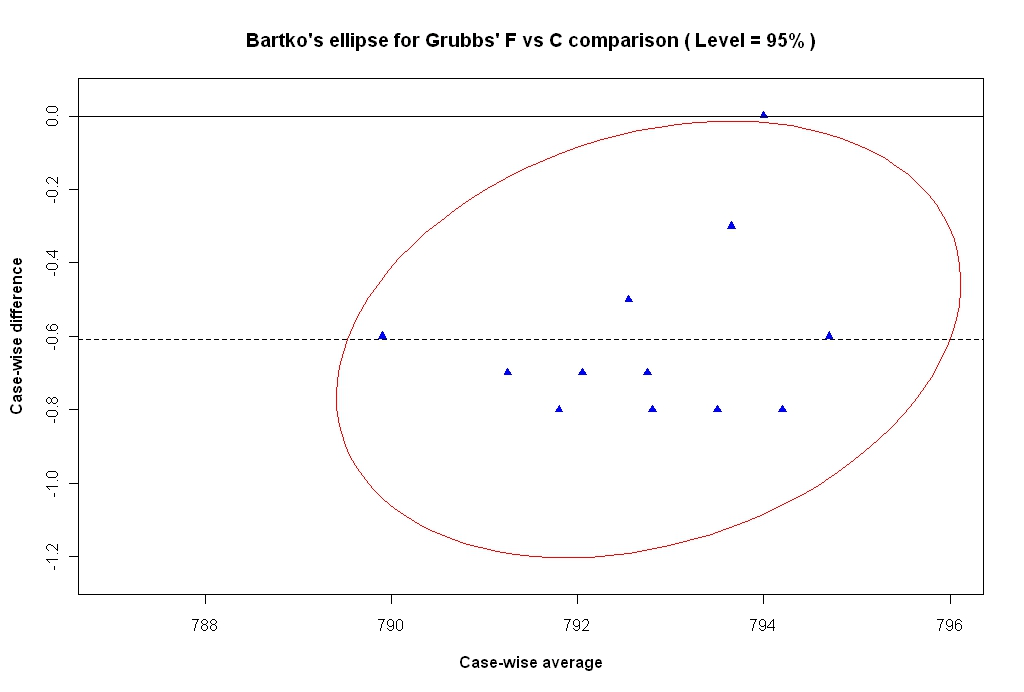
\includegraphics[width=130mm]{images/GrubbsBartko.jpeg}
	\caption{Bartko's Ellipse For Grubbs Data}\label{GrubbsBartko}
\end{figure}

\citet{AltmanEllipse} provides the relevant calculations for the ellipse. This ellipse is intended as a visual
guidelines for the scatter plot, for detecting outliers and to
assess the within- and between-subject variances.

The minor axis relates to the between subject variability, whereas
the major axis relates to the error mean square, with the ellipse
depicting the size of both relative to each other.
Consequently Bartko's ellipse provides a visual aid to determining the
relationship between variances. If $\mbox{var}(a)$ is greater than $\mbox{var}(d)$, the orientation of the ellipse is horizontal. Conversely if $\mbox{var}(a)$ is less than $\mbox{var}(d)$, the orientation of the ellipse is vertical.




%(Furthermore \citet{Bartko}
%proposes formal testing procedures, that shall be discussed in due
%course.)

The Bland-Altman plot for the Grubbs data, complemented by Bartko's ellipse, is depicted in Figure 1.7.
The fourth observation is shown to be outside the bounds of the ellipse, indicating that it is a potential outlier.




The limitations of using bivariate approaches to outlier detection
in the Bland-Altman plot can demonstrated using Bartko's ellipse.
A covariate is added to the `F vs C' comparison that has a
difference value equal to the inter-method bias, and an average
value that markedly deviates from the rest of the average values
in the comparison, i.e. 786. Table 1.8 depicts a $95\%$ confidence
ellipse for this manipulated data set. By inspection of the
confidence interval, we would conclude that this extra
covariate is an outlier, in spite of the fact that this
observation is very close to the inter-method bias as determined by this approach.

\begin{figure}[h!]
	% Requires \usepackage{graphicx}
	\includegraphics[width=130mm]{images/GrubbsBartko2.jpeg}
	\caption{Bartko's Ellipse for Grubbs' data, with an extra covariate.}\label{GrubbsBartko2}
\end{figure}


Importantly, outlier classification must be informed by the logic of the
mechanism that produces the data. In the Bland-Altman plot, the horizontal displacement (i.e. the average) of any
observation is supported by two separate measurements. Any
observation should not be considered an outlier on the basis of a
noticeable horizontal displacement from the main cluster, as in
the case with the extra covariate. Conversely, the fourth
observation, from the original data set, should be considered an
outlier, as it has a noticeable vertical displacement from the
rest of the observations.

%Grubbs' test is a statistical test used for detecting outliers in a
%univariate data set that is assumed to be normally distributed.

%\citet{Grubbs} defined an outlier as a co-variate that appears to
%deviate markedly from other members of the sample in which it
%occurs.
In classifying whether a observation from a univariate data set is
an outlier, many formal tests are available, such as the Grubbs test for outliers. In assessing
whether a covariate in a Bland-Altman plot is an outlier, this
test is useful when applied to the case-wise difference values treated as a
univariate data set. The null hypothesis of the Grubbs test procedure is the absence
of any outliers in the data set. Conversely, the alternative hypotheses is that there is at least one outlier
present.





The test statistic for the Grubbs test ($G$) is the largest
absolute deviation from the sample mean divided by the standard
deviation of the differences,
\begin{equation}
G =  \displaystyle\max_{i=1,\ldots, n}\frac{\left \vert d_i -
	\bar{d}\right\vert}{S_{d}}.
\end{equation}

For the `F vs C' comparison it is the fourth observation gives
rise to the test statistic, $G = 3.64$. The critical value is
calculated using Student's $t$ distribution and the sample size,
\[
U = \frac{n-1}{\sqrt{n}} \sqrt{\frac{t_{\alpha/(2n),n-2}^2}{n - 2
		+ t_{\alpha/(2n),n-2}^2}}.
\]
For this test $U = 0.75$. The conclusion of this test is that the fourth observation in the `F vs C' comparison is an outlier, with $p-$value = 0.003, in accordance with the previous result of Bartko's ellipse.


%========================================================================================== %


\subsection{Bartko's Ellipse}

As an enhancement on the Bland Altman Plot, \citet{Bartko} has
expounded a confidence ellipse for the covariates. \citet{Bartko} proposes
a bivariate confidence ellipse as a boundary for dispersion. The stated purpose is to `amplify dispersion', which presumably is for  the purposes of outlier detection. The orientation of the the ellipse is key to interpreting the results.



%(Furthermore \citet{Bartko}
%proposes formal testing procedures, that shall be discussed in due
%course.)
Bartko states that the ellipse can, inter alia, be used to detect the presence of outliers (furthermore
\citet{Bartko} proposes formal testing procedures, that shall be discussed in due course). 
The Bland-Altman plot for the Grubbs data, complemented by Bartko's ellipse, is depicted in Figure ~\ref{GrubbsBartko1}.
The fourth observation is shown to be outside the bounds of the ellipse, indicating that it is a potential outlier.




The limitations of using bivariate approaches to outlier detection
in the Bland-Altman plot can demonstrated using Bartko's ellipse.
A covariate is added to the `F vs C' comparison that has a
difference value equal to the inter-method bias, and an average
value that markedly deviates from the rest of the average values
in the comparison, i.e. 786. Table 1.8 depicts a $95\%$ confidence
ellipse for this manipulated data set. By inspection of the
confidence interval, a conclusion would be reached that this extra
covariate is an outlier, in spite of the fact that this
observation is wholly consistent with the conclusion of the
Bland-Altman plot.

%\begin{figure}[h!]
%  % Requires \usepackage{graphicx}
%  \includegraphics[width=130mm]{GrubbsBartko2.jpeg}
%  \caption{Bartko's Ellipse For Grubbs' Data, with an extra covariate.}\label{GrubbsBartko2}
%\end{figure}

In the Bland-Altman plot, the horizontal displacement of any point on the plot is supported by two independent measurements. Any point should not be considered an outlier on the basis of a noticeable horizontal displacement from the main cluster, as in the case with the extra co-variate. Conversely, the fourth point, from the original data set, should be considered an
outlier, as it has a noticeable vertical displacement from the rest of the observations.


%\citet{Grubbs} defined an outlier as a co-variate that appears to
%deviate markedly from other members of the sample in which it
%occurs.




Additionally Bartko's ellipse provides a visual aid to determining the
relationship between variances. 
Furthermore, the ellipse provides a visual aid to determining the relationship
between the variance of the means $Var(a_{i})$ and the variance of the differences $Var(d_{i})$. If $\mbox{var}(a)$ is greater than $\mbox{var}(d)$, the orientation of the ellipse is horizontal. Conversely if $\mbox{var}(a)$ is less than $\mbox{var}(d)$, the orientation of the ellipse is vertical. The more horizontal the ellipse, the greater the degree of agreement between the two methods being tested.





%----------------------------------------------------------------------------%



\section{Limits of Agreement}
	Bland and Altman proposed a pair of Limits of agreement, not unlike control limits in control charts. These
	limits are intended to demonstrate the range in which 95\% of the sample data should lie. The Limits of Agreement centre on the
	average difference line and are 1.96 times the standard deviation above and below the average difference line.
	


A third element of the Bland-Altman methodology, an interval known
as `limits of agreement' is introduced in \citet*{BA86}
(sometimes referred to in literature as 95\% limits of agreement). Bland and Altman proposed a pair of Limits of agreement. These
limits are intended to demonstrate the range in which 95\% of the
sample data should lie. The Limits of agreement centre on the
average difference line and are 1.96 times the standard deviation
above and below the average difference line.

Limits of agreement are used to assess whether the two methods of measurement can be used interchangeably. \citet{BA86} refer to
this as the `equivalence' of two measurement methods. The specific purpose of the limits of
agreement must be
established clearly. \citet*{BA95} comment that the limits of agreement `\textit{how
	far apart measurements by the two methods were likely to be for
	most individuals}', a definition echoed in their 1999 paper:

\begin{quote}"We can then say that nearly all pairs
	of measurements by the two methods will be closer together than
	these extreme values, which we call 95\% limits of agreement.
	These values define the range within which most differences
	between measurements by the two methods will lie."
\end{quote}

	
	The limits of agreement (LoA) are computed by the following
	formula:
	\[
	LoA = \bar{d} \pm 1.96 s_{d}
	\]
	with $\bar{d}$ as the estimate of the inter method bias, $s_{d}$
	as the standard deviation of the differences and 1.96 (sometimes rounded to 2) is the 95\%
	quantile for the standard normal distribution. The limits of agreement methodology assumes a constant level of bias throughout the range of measurements.
Limits of agreement are used to assess whether the two methods of
measurement can be used interchangeably. \citet{BA86} refer to
this as the `equivalence' of two measurement methods. The specific question to which limits of agreement are intended as the answer to must be established clearly. \citet*{BA95} comment that the limits of agreement show `how	far apart measurements by the two methods were likely to be for most individuals', a definition echoed in their 1999 paper:



Importantly the authors recommend prior determination of what would constitute acceptable
agreement, and that sample sizes should be predetermined to give an accurate conclusion. However \citet{mantha} highlight inadequacies in the correct application of limits of agreement, resulting in contradictory estimates of limits of agreement in various papers.

Calculation of the limits of agreement relies on the assumption that the case-wise differences are normally distributed.
The calculation removes a lot of the variation between subjects,  leaving measurement error, which is likely to be normally distributed. (\citet{BA99} remark that this assumption is easy to check using a normal plot.) 
	How this relates the overall population is unclear. It seems that it depends on an expert to decide whether or not the range of
	differences is acceptable. 
	If one method is sometimes higher, and sometimes the other method is higher, the average of the differences will be close to zero.
	If it is not close to zero, this indicates that the two assay methods are producing different results systematically.
	
The difference are assumed to be normally distributed, although the measurements themselves are not assumed to follow any distribution. Therefore the authors argue that the 95\% of differences are expected to lie within these limits. This assumption is justified because variation between subjects has been removed, leaving only measurement error \citep{BA86}. There are formal methodologies to test whether this assumption holds.

The limits of agreement methodology assumes a constant level of bias throughout the range of measurements. Importantly the authors recommend prior determination of what would and would constitute acceptable
agreement, and that sample sizes should be predetermined to give an accurate conclusion. 

\begin{quote}
	``How far apart measurements can be without causing difficulties
	will be a question of judgment. Ideally, it should be defined in
	advance to help in the interpretation of the method comparison and
	to choose the sample size \citep{BA86}".
\end{quote}

However \citet{mantha} highlights inadequacies in the correct application of limits of agreement, resulting in contradictory estimates for limits of agreement in various papers.

For the Grubbs `F vs C' comparison, these limits
of agreement are calculated as -0.132 for the upper bound, and
-1.08 for the lower bound. Figure ~\ref{GrubbsBAplot-noLOA} shows the resultant
Bland-Altman plot, with the limits of agreement shown in dashed
lines.


\begin{figure}[h!]
	\begin{center}
		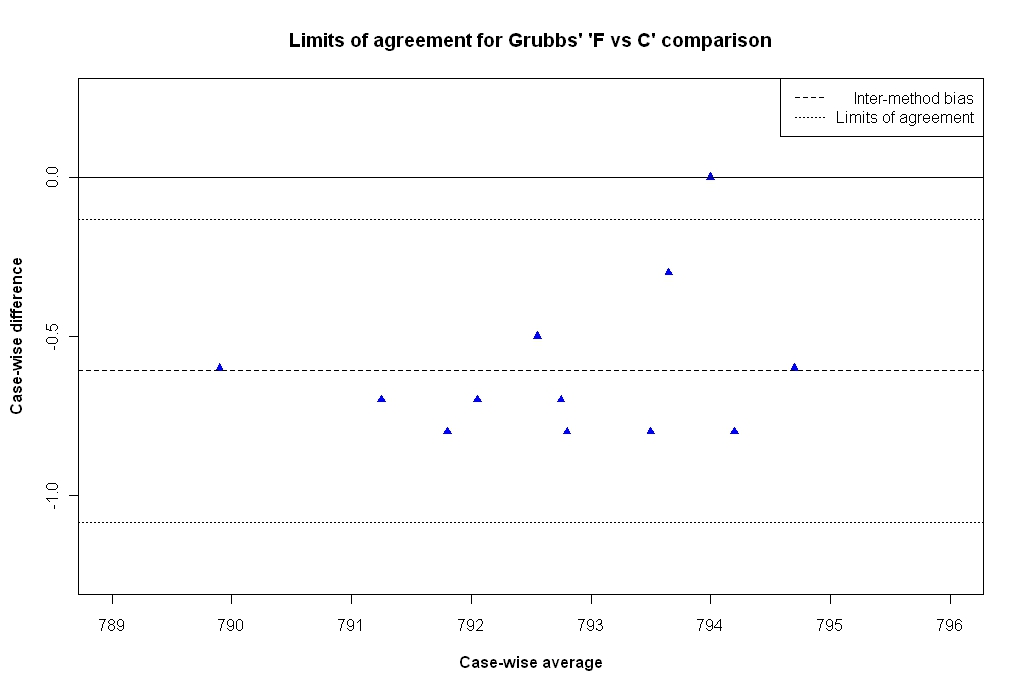
\includegraphics[width=125mm]{images/GrubbsBAplot-LOA.jpeg} 
		\caption{Bland-Altman plot with limits of agreement}
		\label{GrubbsBAplot-noLOA}
	\end{center}
\end{figure}
\newpage

%But as \citet*{BA86} point out this may not be the case. Variants of the limits of agreement that overcome this
% problem shall be introduced in due course.


\section{Interpretation of Limits Of Agreement}
It must be established
clearly the specific purpose of the limits of agreement.
\citet*{BA95} comment that the limits of agreement \emph{how far
	apart measurements by the two methods were likely to be for most
	individuals.}, a definition echoed in their 1999 paper:
\begin{quote} We can then say that nearly all pairs
	of measurements by the two methods will be closer together than
	these extreme values, which we call 95\% limits of agreement.
	These values define the range within which most differences
	between measurements by the two methods will lie\citep{BA99}.
\end{quote}
\citet{BXC2008} offers an alternative, more specific,  definition of
the limits of agreement \emph{"a prediction interval for the
	difference between future measurements with the two methods on a
	new individual."} \citet{luiz} describes them as tolerance limits.



%\begin{quote}
%``How far apart measurements can be without causing difficulties
%will be a question of judgment. Ideally, it should be defined in
%advance to help in the interpretation of the method comparison and
%to choose the sample size \citep{BA86}".
%\end{quote}


For the Grubbs `F vs C' comparison, these limits
of agreement are calculated as -0.132 for the upper bound, and
-1.08 for the lower bound. Figure 1.9 shows the resultant
Bland-Altman plot, with the limits of agreement shown in dashed
lines.


%----------------------------------------------------------------------------%

\subsection{Appropriate Use of Limits of Agreement}
Importantly \citet{BA99} makes the following point:
\begin{quote}These estimates are meaningful only if we can assume
	bias and variability are uniform throughout the range of
	measurement, assumptions which can be checked graphically.
\end{quote}

The import of this statement is that, should the Bland-Altman plot indicate that these assumptions are not met, then their entire methodology, as posited thus far, is inappropriate for use in a method comparison study. Again, in the context of potential outlier in the Grubbs data (figure 1.2), this raises the question on how to correctly continue.
%
%Carstensen attends to the issue of repeated data, using the
%expression replicate to express a repeated measurement on a
%subject by the same methods. Carstensen formulates the data as
%follows Repeated measurement - Arrangement of data into groups,
%based on the series of results of each subject.







Several problems have been highlighted regarding Limits of
Agreement. One is the somewhat arbitrary manner in which they are
constructed. While in essence a confidence interval, they are not
constructed a such. They are designed for future values.

The formulation is also heavily influenced by outliers. An Example
in \citet*{BA83} demonstrates the effect of recalculating without
a particular outlier. Refering to the VCF data set in the same
paper, there is more than one outlier.


\subsection{Formal definition of Limits of Agreement}
\citet{BA99} note the similarity of limits of agreement to confidence intervals, but are clear that they are not the same
thing. Interestingly, they simply describe the limits as `being like a reference interval', offering no elaboration.

Limits of agreement have very similar construction to Shewhart control limits. The Shewhart chart is a well known graphical
methodology used in statistical process control. Consequently there is potential for misinterpreting the limits of agreement as
they were Shewhart control limits. Importantly the parameters used to determine the Shewhart limits are time ordered, based on the process's historical values, a key difference with Bland-Altman limits of agreement.

\citet{BXC2008} regards the limits of agreement as a prediction interval for the difference between future measurements with the
two methods on a new individual, but states that it does not fit the formal definition of a prediction interval, since the definition does not consider the errors in estimation of the parameters. Prediction intervals, which are often used in regression analysis, are estimates of an interval in which future observations will fall, with a certain probability, given what has
already been observed. \citet{BXC2008} offers an alternative formulation, a $95\%$ prediction interval for the difference

\[
\bar{d} \pm t_{(0.025, n-1)}s_{d} \sqrt{1+\frac{1}{n}}
\]

\noindent where $n$ is the number of subjects. Carstensen is careful to consider the effect of the sample size on the interval
width, adding that only for 61 or more subjects is the quantile less than 2.

\citet{luiz} describes limits of agreement as tolerance limits. A
tolerance interval for a measured quantity is the interval in
which a specified fraction of the population's values lie, with a
specified level of confidence. \citet{luiz} offers an alternative description of limits of agreement, this time as tolerance limits. A tolerance interval for a measured quantity is the interval in which a specified fraction of the population's values lie, with a specified level of confidence. \citet{Barnhart} describes them as a probability interval, and offers a clear description of how they should be used; `\textit{if the absolute limit is less than an acceptable difference $d_{0}$, then the agreement between the two methods is deemed satisfactory}'.

The prevalence of contradictory definitions of what limits of agreement strictly are will inevitably attenuate the poor standard of reporting using limits of agreement, as mentioned by \citet{mantha}.

%At least 100 historical
%values must be used to determine the acceptable value (i.e the
%process mean) and the process standard deviation. The principle
%that the mean and variance of a large sample of a homogeneous
%population is a close approximation of the population's mean and
%variance justifies this.

%\begin{figure}[h!]
%\begin{center}
%  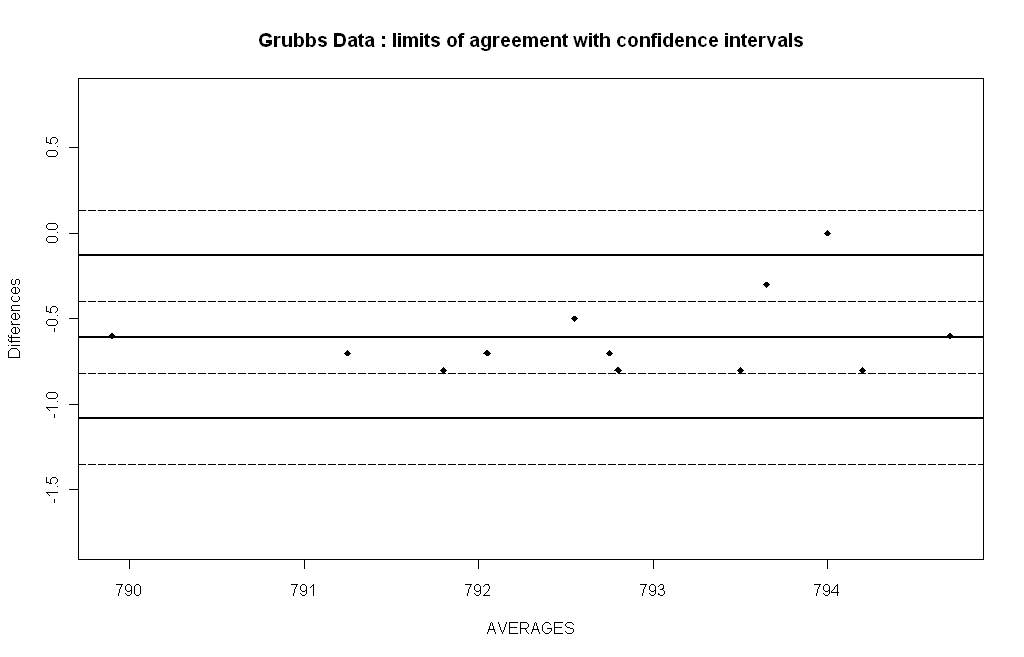
\includegraphics[width=125mm]{GrubbsLOAwCIs.jpeg}
%  \caption{Limits of agreement with confidence intervals}\label{LOAwCIs}
%\end{center}
%\end{figure}

%\newpage
%\section{Agreement Indices}
%\citet{Barnhart} provided an overview of several agreement
%indices, including the limits of agreement. Other approaches, such
%as mean squared deviation, the tolerance deviation index and
%coverage probability are also discussed.


%At least 100 historical
%values must be used to determine the acceptable value (i.e the
%process mean) and the process standard deviation. The principle
%that the mean and variance of a large sample of a homogeneous
%population is a close approximation of the population's mean and
%variance justifies this.

\citet{BA99} note the similarity of limits of agreement to
confidence intervals, but are clear that they are not the same thing. Interestingly, they describe the limits as `\textit{being like a reference interval}'.

Limits of agreement have very similar construction to Shewhart control limits. The Shewhart chart is a well known graphical
methodology used in statistical process control. Consequently there is potential for misinterpreting the limits of agreement as if equivalent to Shewhart control limits. Importantly the parameters used to determine the Shewhart limits are not based on any sample used for an analysis, but
on the process's historical values, a key difference with
Bland-Altman limits of agreement.

\citet{BXC2008} regards the limits of agreement as a prediction interval for the difference between future measurements with the two methods on a new individual, but states that it does not fit
the formal definition of a prediction interval, since the definition does not consider the errors in estimation of the
parameters. Prediction intervals, which are often used in regression analysis, are estimates of an interval in which future
observations will fall, with a certain probability, given what has already been observed. \citet{BXC2008} offers an alternative formulation, a $95\%$ prediction interval for the difference
\[
\bar{d} \pm t_{(0.975, n-1)}s_{d} \sqrt{1+\frac{1}{n}}
\]

Various other interpretations as to how limits of agreement should properly be defined. 

The prevalence of contradictory definitions of what limits of agreement strictly are will inevitably attenuate the poor standard of reporting using limits of agreement, as discussed by \citet{mantha}.

%\begin{figure}[h!]
%\begin{center}
%  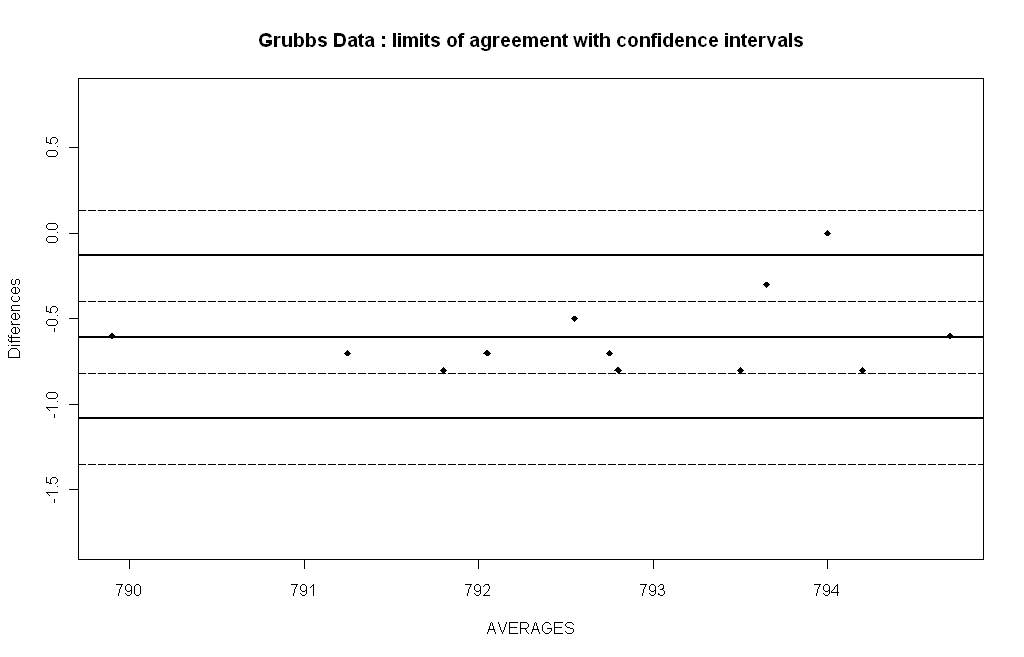
\includegraphics[width=125mm]{GrubbsLOAwCIs.jpeg}
%  \caption{Limits of agreement with confidence intervals}\label{LOAwCIs}
%\end{center}
%\end{figure}

\section{Inferences on Bland-Altman estimates}
	The limits of agreement are estimates derived from the sample
	studied, and will differ from values relevant to the whole
	population. \citet*{BA86} advance a formulation for confidence
	intervals of the inter-method bias and the limits of agreement.
	These calculations employ quantiles of the `t' distribution with
	$n -1$ degrees of freedom.
	
	%This page also shows the standard deviation (SD) of the
	%differences between the two assay methods. The SD value is used to
	%calculate the limits of agreement, computed as the mean bias plus
	%or minus 1.96 times its SD.
%	\citet*{BA99} advises on how to calculate confidence intervals for the inter-method bias and limits of agreement.
	For the inter-method bias, the confidence interval is a simply that of a mean: $\bar{d} \pm t_{(\alpha/2,n-1)} S_{d}/\sqrt{n}$.
	The confidence
	intervals and standard error for the limits of agreement follow from the variance of the limits of agreement, which is shown to be
	
	\[
	\mbox{Var}(LoA) = (\frac{1}{n}+\frac{1.96^{2}}{2(n-1)})s_{d}^{2}.
	\]
	
	If $n$ is sufficiently large this can be following approximation can be used
	\[
	\mbox{Var}(LoA) \approx 1.71^{2}\frac{s_{d}^{2}}{n}.
	\]
	Consequently the standard errors of both limits can be approximated as $1.71$ times the standard error of the differences.
	
	A $95\%$ confidence interval can be determined, by means of the \emph{t} distribution with $n-1$ degrees of freedom. However, \citet*{BA99} comment that such calculations  may be `somewhat optimistic' on account of the associated assumptions not being realized.
	
	%\section{Small Sample Sizes} The limits of agreement are
	%estimates derived from the sample studied, and will differ from
	%values relevant to the whole population, hence the importance of a
	%suitably large sample size. A different sample would give
	%different limits of agreement. Student's t-distribution is a well
	%known probability distribution used in statistical inference for
	%normally distributed populations when the sample size is small
	%\citep{student,Fisher3}. Consequently, using 't' quantiles , as
	%opposed to standard normal quantiles, may give a more appropriate
	%calculation for limits of agreement when the sample size is small.
	%For sample size $n=12$ the `t' quantile is 2.2 and the limits of
	%agreement are (-0.074,-1.143).
	


%%%%%%%%%%%%%%%%%%%%%%%%%%%%%%%%%%%%%%%%%%%%%%%%%%%%%%%%%%%%%%%%%%%%%%%%%%%%%%%%%%%%%%
\newpage
		
\section{Formal Testing}
The Bland Altman plot is a simple tool for inspection of the data,
but in itself it offers no formal testing procedure in this regard. To this end, the approach proposed by \citet{BA83} is a formal test on the Pearson correlation coefficient  of casewise differences and means ($\rho_{AD}$). According to the authors, this test is equivalent to a well established tests for equality of variances, known as the `Pitman Morgan Test' \citep{Pitman,
	Morgan}.

For the Grubbs data, the correlation coefficient estimate ($r_{AD}$) is 0.2625, with a 95\% confidence interval of (-0.366,
0.726) estimated by Fishers 'r to z' transformation \citep{Cohen}. The null hypothesis ($\rho_{AD}$ =0) would fail to be rejected.
Consequently the null hypothesis of equal variances of each method would also fail to be rejected.

There has no been no further mention of this particular test in the subsequent article published by Bland and Altman, although
\citet{BA99} refers to Spearmans' rank correlation coefficient. \citet{BA99} comments `we do not see a
place for methods of analysis based on hypothesis testing'. \citet{BA99} also states that consider structural equation models
to be inappropriate.
%=================================================================%
\section{Variations of the Bland-Altman Plot} 
Importantly \citet{BA99} makes the following point:
\begin{quote}These estimates are meaningful only if we can assume
	bias and variability are uniform throughout the range of
	measurement, assumptions which can be checked graphically.
\end{quote}

The import of this statement is that , should the Bland Altman plot indicate that these assumptions are not met, then their
entire methodology, as posited thus far, is inappropriate for use
in a method comparison study. Again, in the context of potential
outlier in the Grubbs data (figure 1.2), this raises the question
on how to correctly continue. Due to limitations of the conventional difference plot, a series of alternative formulations for the Bland-Altman approach have been proposed.
Referring to the assumption that bias and variability are constant across the range
of measurements, \citet{BA99} address the case where there is an increase in variability as the magnitude increases. They remark 	that it is possible to ignore the issue altogether, but the limits of agreement would be wider apart than necessary when just lower magnitude measurements are considered. Conversely the limits would be too narrow should only higher magnitude measurements be used. To address the issue, they propose the logarithmic transformation of the data. The plot is then formulated as the difference of paired log values against their mean. Bland and Altman acknowledge that this is not easy to interpret, and may not be suitable in all cases.

\citet{BA99} offers two variations of the Bland-Altman plot that are intended to overcome potential problems that the conventional
plot would inappropriate for. The first variation is a plot of case-wise differences as percentage of averages, and is
appropriate when there is an increase in variability of the differences as the magnitude increases. The second variation is a
plot of case-wise ratios as percentage of averages. This will remove the need for $log$ transformation. This approach is useful
when there is an increase in variability of the differences as the magnitude of the measurement increases. \citet{Eksborg} proposed
such a ratio plot, independently of Bland and Altman. \citet{Dewitte} commented on the reception of this article by saying `Strange to say,this report has been overlooked'.
	
	%	%----------------------------------------------------------------%
	%	\section{Dewitte et al }
	%	\begin{quote}When the standard deviation increases with concentration, Bland and Altman recommend a logarithmic y scale, whereas others propose a percent y scale (Pollock et al, 2002). Although generally there is not much difference in effect between using percentages and using a log transformation of the data, we prefer the percent plot (except when data extend over several orders of magnitude) because numbers can be read directly from the plot without the need for back-transformation.
	%	\end{quote}
	%	
	%	\begin{verbatim}
	%	absolute - small range
	%	percentage - medium range
	%	log scale - large range
	%	\end{verbatim}
	%==================================================== %
	
\section{Limits of Agreement for Replicate Measurements}

Computing limits of agreement features prominently in many method comparison studies since the publication of \citet{BA86}.
\citet{BA99} addresses the issue of computing LoAs in the presence of replicate measurements, suggesting several computationally simple approaches. When repeated measures data are available, it is desirable to use
all the data to compare the two methods. However, the original Bland-Altman method was developed for two sets of measurements done on one occasion, and so this approach is not suitable for replicate measures data. However, as a naive analysis, it may be used to explore the data because of the simplicity of the method.
In addition to \citet{BA99}, \citet{BXC2008} computes the limits of agreement to the case with replicate measurements by using LME models, an approach that will be discussed in due course.


The limits of agreement methodology assumes a constant level of bias throughout the range of measurements. As \citet*{BA86} point out this may not be the case. Bland and Altman advises on how to calculate of confidence intervals for the inter-method bias and
the limits of agreement. Importantly the authors recommend prior determination of what would and would constitute acceptable
agreement, and that sample sizes should be predetermined to give an accurate conclusion.

\begin{quote}
	`How far apart measurements can be without causing difficulties
	will be a question of judgment. Ideally, it should be defined in
	advance to help in the interpretation of the method comparison and
	to choose the sample size.'\citep{BA86}
\end{quote}



\subsection{Confidence Intervals and Standard Error}
\citet*{BA99} argue that it is possible to estimate confidence
intervals and standard error, if it is assumed that the
differences approximately follow a normal distribution,

\begin{equation}
\mbox{Var}(LoA) = (\frac{1}{n}+\frac{1.96^{2}}{2(n-1)})S_{d}^{2}.
\end{equation}

If $n$ is sufficiently large this can be following approximation
can be used
\begin{equation}
\mbox{Var}(LoA) \approx 1.71^{2}\frac{S_{d}^{2}}{n}.
\end{equation}
Consequently the standard errors of both limits can be
approximated as $1.71 S.E.(\bar{d})$

A $95\%$ confidence interval can be determined, by means of the
\emph{t} distribution with $n-1$ degrees of freedom. \citet*{BA99} comment that such calculations  may be `somewhat
optimistic' on account of the associated assumptions not being
realized.

%This page also shows the standard deviation (SD) of the
%differences between the two assay methods. The SD value is used to
%calculate the limits of agreement, computed as the mean bias plus
%or minus 1.96 times its SD.
%----------------------------------------------------------------------------%
%	\subsection{Appropriate Use of Limits of Agreement}
%	
%	Carstensen attends to the issue of repeated data, using the
%	expression replicate to express a repeated measurement on a
%	subject by the same methods. Carstensen formulates the data as
%	follows Repeated measurement - Arrangement of data into groups,
%	based on the series of results of each subject.
%	



\subsection{Model Specification}
The model underpinning the Bland-Altman approach can be presented as follows:



The case-wise differences $d_i = x_i - y_i$
\[
\Sigma = \left( \begin{array}{cc}
\sigma^2_1 + \sigma^2_2 &  \frac{1}{2}(\sigma^2_1 - \sigma^2_2) \\
\frac{1}{2}(\sigma^2_1 - \sigma^2_2) &   \sigma^2_b + \frac{1}{4}(\sigma^2_1 + \sigma^2_2)
\end{array}\right)
\]







	

\section{Prevalence of the Bland-Altman plot}
	%---------------------------------------------%

\citet*{BA86}, which further develops the Bland-Altman methodology,
was found to be the sixth most cited paper of all time by the
\citet{BAcite}. \cite{Dewitte} describes the rate at which
	prevalence of the Bland-Altman plot has developed in scientific
	literature. \citet{Dewitte} reviewed the use of Bland-Altman plots
	by examining all articles in the journal `Clinical Chemistry'
	between 1995 and 2001. This study concluded that use of the
	Bland-Altman plot increased over the years, from 8\% in 1995 to
	14\% in 1996, and 31-36\% in 2002.
	
	The Bland-Altman Plot has since become expected, and
	often obligatory, approach for presenting method comparison
	studies in many scientific journals \citep{hollis}. Furthermore
	\citet{BritHypSoc} recommend its use in papers pertaining to
	method comparison studies for the journal of the British
	Hypertension Society.
	

% %	\section{Bland Altman Plots In Literature}
	\citet{mantha} contains a study the use of Bland Altman plots of
	44 articles in several named journals over a two year period. 42
	articles used Bland Altman's limits of agreement, wit the other
	two used correlation and regression analyses. \citet{mantha}
	remarks that 3 papers, from 42 mention predefined maximum width
	for limits of agreement which would not impair medical care.
	
	The conclusion of \citet{mantha} is that there are several
	inadequacies and inconsistencies in the reporting of results ,and
	that more standardization in the use of Bland Altman plots is
	required. The authors recommend the prior determination of limits
	of agreement before the study is carried out. This contention is
	endorsed by \citet{lin}, which makes a similar recommendation for
	the sample size, noting that\emph{sample sizes required either was
		not mentioned or no rationale for its choice was given}.
	
	\begin{quote}
		In order to avoid the appearance of "data dredging", both the
		sample size and the (limits of agreement) should be specified and
		justified before the actual conduct of the trial. \citep{lin}
	\end{quote}
	
	\citet{Dewitte} remarks that the limits of agreement should be
	compared to a clinically acceptable difference in measurements.
	%%%%%%%%%%%%%%%%%%%%%%%%%%%%%%%%%%%%%%%%%%%%%%%%%%%%%%%%%%%%%%%%%%%%%%%%%

	%%%%%%%%%%%%%%%%%%%%%%%%%%%%%%%%%%%%%%%%%%%%%%%%%%%%%%%%%%%%%%%%%%%%%%%%%
	%4 Inappropriate assessment of Agreement       %%%%%%%%%%%%%%%%%%%%%%%%%%
	%%%%%%%%%%%%%%%%%%%%%%%%%%%%%%%%%%%%%%%%%%%%%%%%%%%%%%%%%%%%%%%%%%%%%%%%%
	
	\section{Analysis of Variance }
	
	\citet{BXC2004} presents a model to describe the relationship between a value of measurement and its
	real value. The non-replicate case is considered first, as it is the context of the Bland Altman plots. This model assumes that inter-method bias is the only difference between the two methods.
	
	A measurement $y_{mi}$ by method $m$ on individual $i$ is formulated as follows;
	\begin{equation}
	y_{mi}  = \alpha_{m} + \mu_{i} + e_{mi} \qquad  e_{mi} \sim
	\mathcal{N}(0,\sigma^{2}_{m})
	\end{equation}
	The differences are expressed as $d_{i} = y_{1i} - y_{2i}$. For the replicate case, an interaction term $c$ is added to the model, with an associated variance component. All the random effects are assumed independent, and that all replicate measurements are assumed to be exchangeable within each method.
	
	\begin{equation}
	y_{mir}  = \alpha_{m} + \mu_{i} + c_{mi} + e_{mir}, \qquad  e_{mi}
	\sim \mathcal{N}(0,\sigma^{2}_{m}), \quad c_{mi} \sim \mathcal{N}(0,\tau^{2}_{m}).
	\end{equation}
	%----
	
	Of particular importance is terms of the model, a true value for item $i$ ($\mu_{i}$).  The fixed effect of Roy's model comprise of an intercept term and fixed effect terms for both methods, with no reference to the true value of any individual item. 
	%A distinction can be made between the two models: Roy's model is a standard LME model, whereas Carstensen's model is a more complex additive model.
	
	\bigskip
	
\bibliographystyle{chicago}
\bibliography{DB-txfrbib}
\end{document}
